\section{System Design\label{sec:systemDesign}}
In this section, we provide an overview of visual encoding for blazar data and the visual exploration framework of TimeTubesX.
% We introduce a 3D tube expression of our previous TimeTubes~\cite{Fujishiro2018} into TimeTubesX.

\begin{figure}[tb]
    \begin{minipage}{0.34\linewidth}
        \centering
        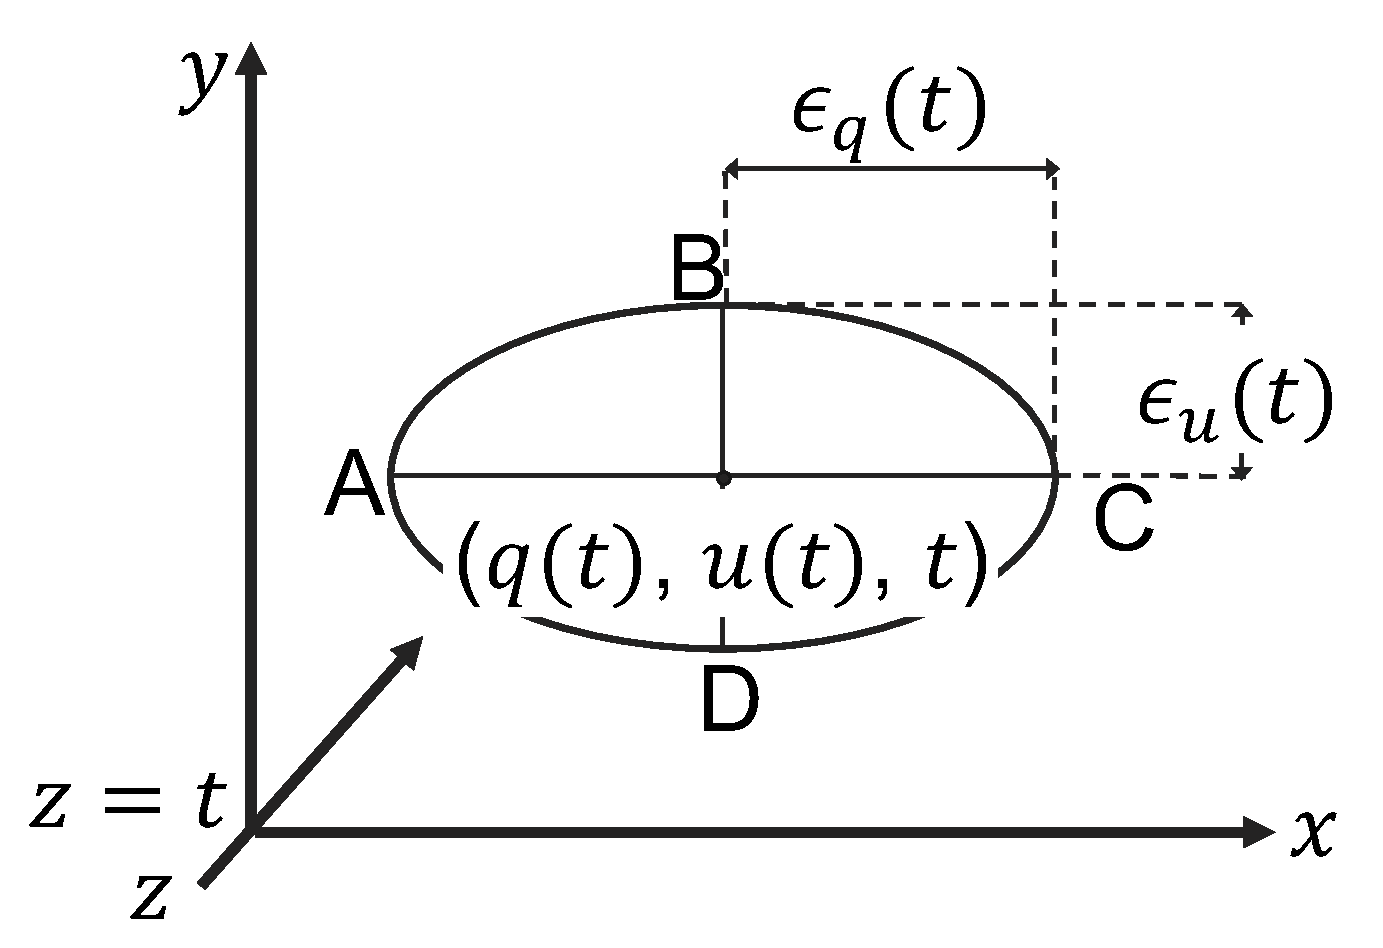
\includegraphics[width=.99\linewidth]{vgtc_journal_latex/figures/howtoplot.pdf}
    \end{minipage}
    \begin{minipage}{0.26\linewidth}
        \centering
        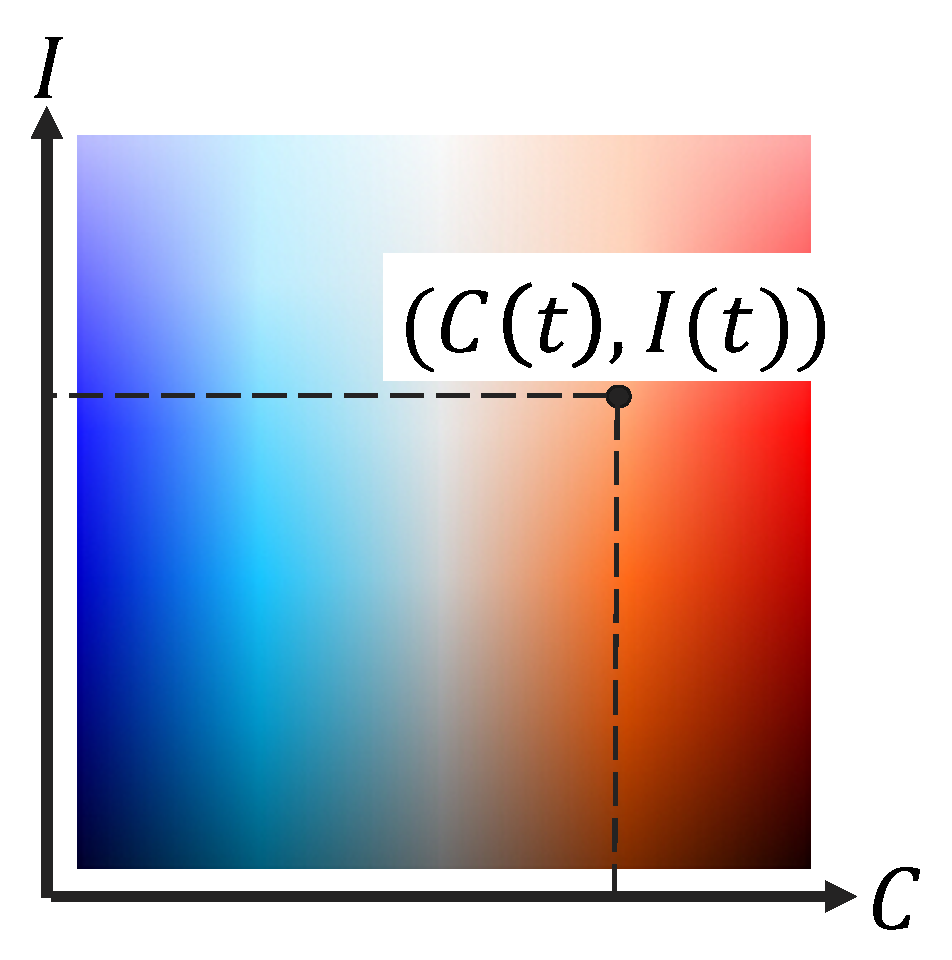
\includegraphics[width=.99\linewidth]{vgtc_journal_latex/figures/colormap.pdf}
    \end{minipage}
    \begin{minipage}{0.36\linewidth}
        \centering
        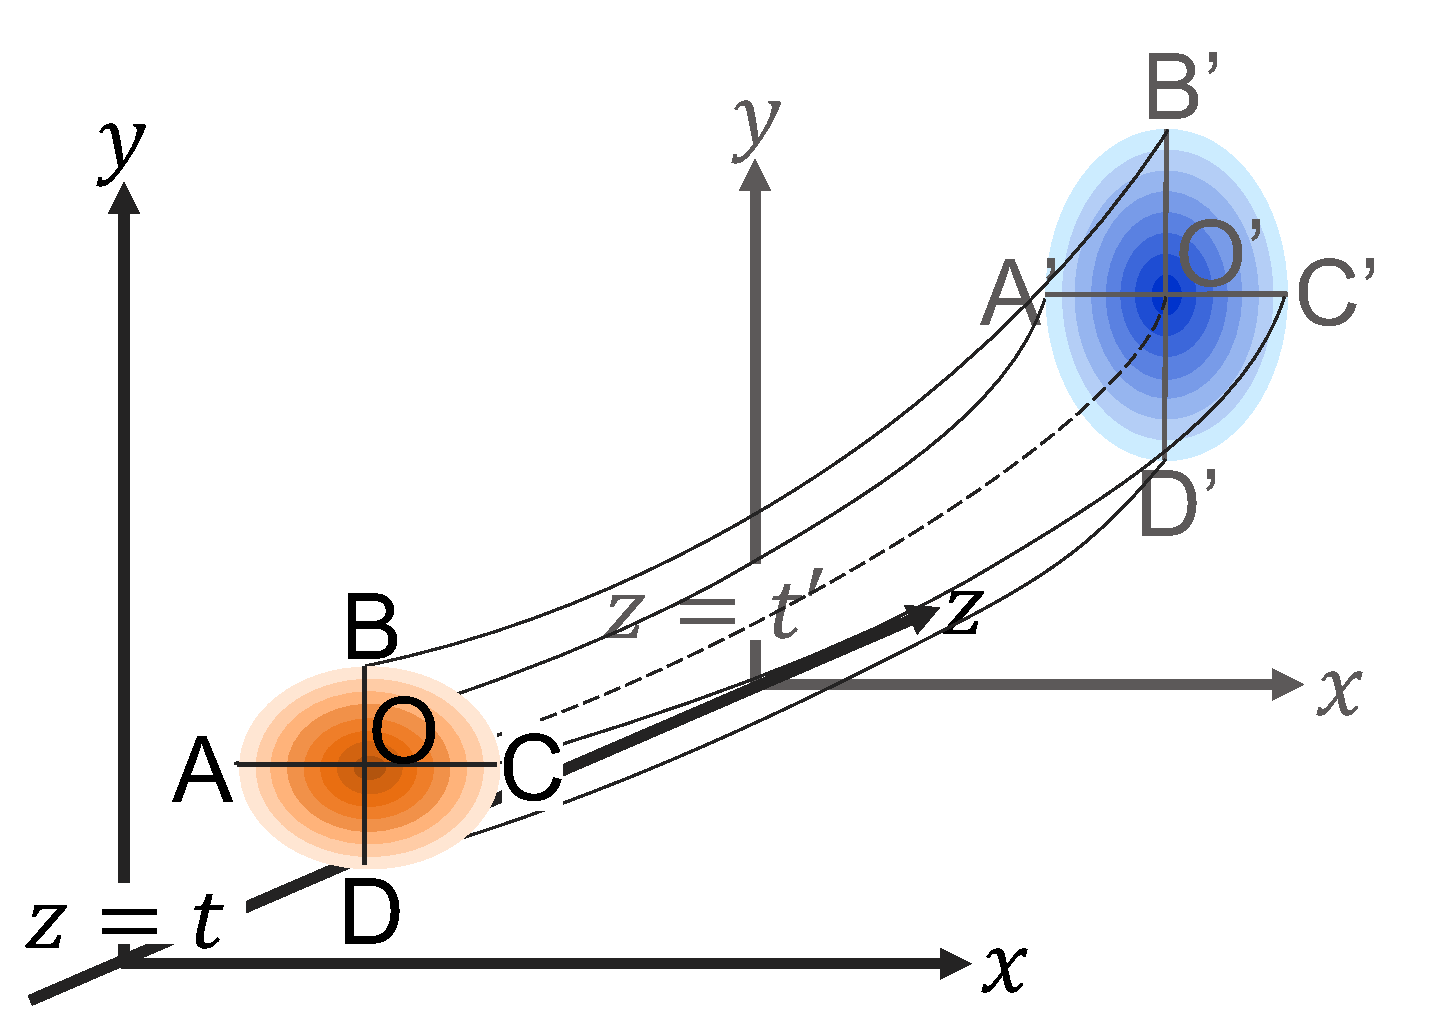
\includegraphics[width=.99\linewidth]{vgtc_journal_latex/figures/howtotube.pdf}
    \end{minipage}
    \begin{minipage}{0.34\linewidth}
        \centering
        \footnotesize{\sf (a)}
        \end{minipage}
    \begin{minipage}{0.26\linewidth}
        \centering
        \footnotesize{\sf (b)}
    \end{minipage}
    \begin{minipage}{0.36\linewidth}
        \centering
        \footnotesize{\sf (c)}
    \end{minipage}
    \caption{Spatial mapping in the TimeTubes view. 
    (a)~Observation values of polarization decide the position and shape of an ellipse;
    (b)~observation values of intensity and color colorize the ellipse with reference to a colormap; and
    (c)~the neighboring ellipses are smoothly connected in chronological order to yield a tube shape.}
    \label{fig:howtoplot}
\end{figure}
\subsection{Visual Encoding for Blazar Data}\label{sec:VisualEncoding}
\begin{figure*}
    \centering
    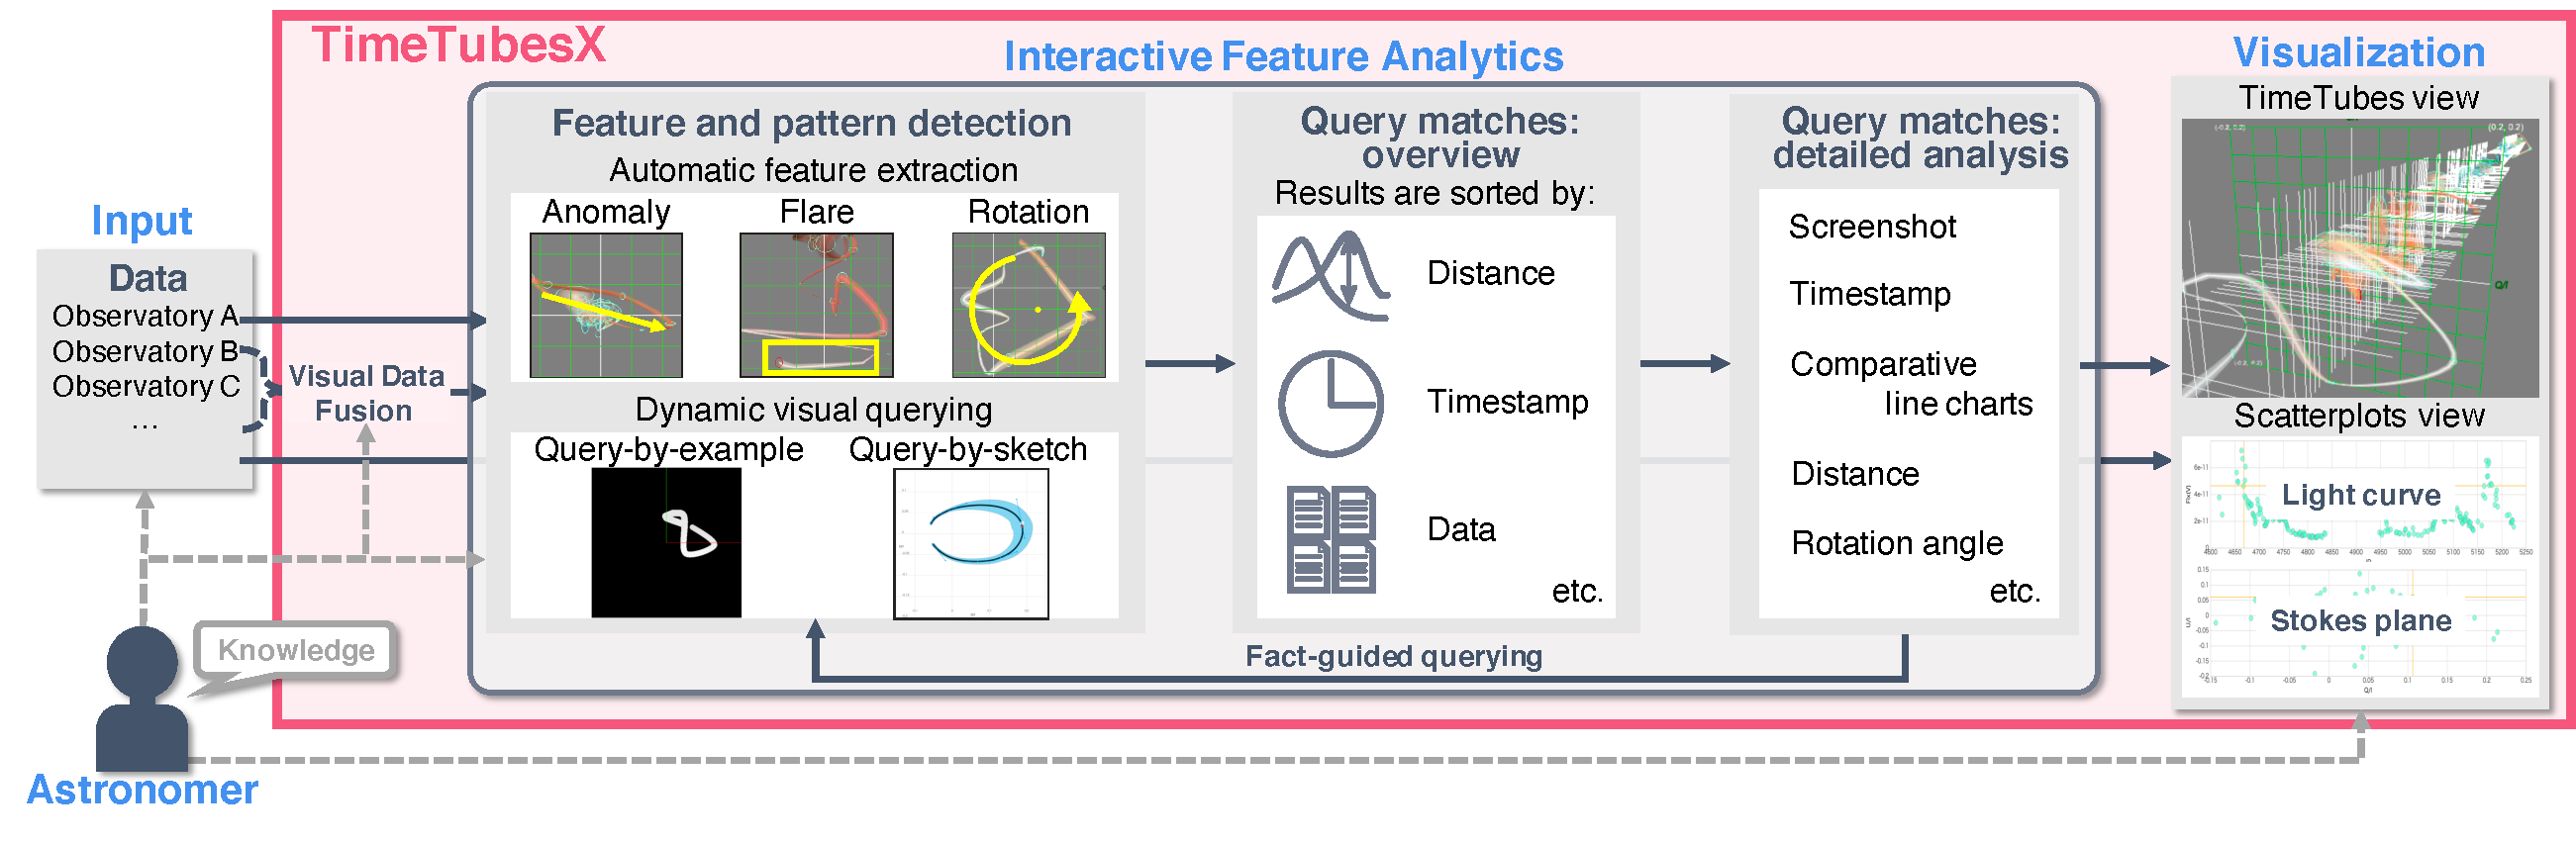
\includegraphics[width=.99\linewidth]{vgtc_journal_latex/figures/workflowGray.pdf}
    \caption{The visual exploration framework of TimeTubesX. Users can load multiple datasets into a single exploration session through visual data fusion. (A)~Users specify a query to extract features of interest; (B)~query results are sorted by relevance; (C)~individual results can be analyzed in high detail and compared to each other; (D)~an extraction result can be re-used as an input for a new visual query; and (E)~users can visually explore the results in the TimeTubes and scatterplots views.}
    \label{fig:framework}
\end{figure*}
Astronomers have used three animated scatterplots with error bars to visualize their multi-dimensional, time-dependent observations (see the accompanying video): one for time variation of $I$, termed \textit{light curve}, another for the Stokes plane, and a third for the correlation between $I$ and $C$.
During the animation, individual observations are highlighted in red in order of observation.
% The animated scatterplots are comprised of three scatterplots, one for the time variation of $I$, termed \textit{light curve}, another for the Stokes plane, and a third for the correlation between $I$ and $C$.
% The \textit{light curve} (\autoref{fig:traditionalMethod}~(a)) is the most important plot for astronomers, and shows the variation of $I$ over time. 
% (b) shows the Stokes plane,
% while (c) displays the correlation between $I$ and $C$.
%

Instead of animating multiple 2D scatterplots,
TimeTubesX expresses blazar observations as a single 3D volumetric tube. 
In the following part, we give a short overview of the \emph{TimeTubes view}, which was originally proposed in our previous work~\cite{Fujishiro2018}.
% We call the view of the 3D volumetric tube \emph{TimeTubes view}.
The TimeTubes view %, that is explained in Fig.~\ref{fig:howtoplot}, 
allows users to see correlations and variations of variables over time at a glance, as illustrated in Fig.~\ref{fig:framework}~(E).
In the current version, users need to import .csv files with column names from their local environment into TimeTubesX.
%as shown in TimeTubes view in the lower right of \autoref{fig:framework}.
%
We use a left-handed coordinate system to assign $q$ and $u$ to the $x$ and $y$ axes, respectively, and time $t$ to the $z$ axis.
%of the visualization domain, $u$ to $y$ axis, and $t$ to $z$ axis.
We encode the polarization parameters ($q$, $u$, $\epsilon_q$, $\epsilon_u$) at each timestamp $t$ as an ellipse centered at the point $(x, y, z) = (q(t), u(t), t)$ with a width of $2\epsilon_q(t)$ and a height of $2\epsilon_u(t)$, as depicted in Fig.~\ref{fig:howtoplot}~(a). 
Therefore, the $x$--$y$ location of an ellipse indicates the polarization at a certain time stamp, while the size of the ellipse indicates the uncertainty of the measurement.
To properly render a 3D tube, we set the value range of the Stokes plane in the TimeTubes view with reference to the standard deviations of $q$ and $u$ in the datasets. 
In the current TimeTubes view, we empirically map a single day to a single voxel along the $z$ axis.
%
We colorize the ellipses according to $I(t)$ and $C(t)$ as based on a user-defined 2D colormap (Fig.~\ref{fig:howtoplot}~(b)). 
The TimeTubes view connects neighboring ellipses in chronological order, using centripetal Catmull-Rom splines to form a 3D volumetric tube (Fig.~\ref{fig:howtoplot}~(c)). 
To further reflect the reliability of the observations, the TimeTubes view offers an adjustable opacity transfer function.
Multiple concentric tubes with different transparencies (i.e., higher opacities for inner tubes) compose a single tube that allows users to intuitively perceive the uncertainties of observations.
Specifically, a time interval with small errors looks like an opaque tube, whereas a time interval with large errors looks more semi-transparent and fuzzy.

Compared with the initial animated scatterplots,
the TimeTubes view provides more uncertainty-aware visual encoding for the analysis of blazar behaviors (\textbf{T1}).
Astronomers do not need to scrutinize multiple plots to understand correlations between variables
or move sliders back and forth %in time 
to track time variations.

%
% Refer to our previous paper~\cite{Fujishiro2018} for more details about the visual encoding of TimeTubes. % interactive exploration functions. %, which were designed according to Shneiderman's Visual Information Seeking Mantra~\cite{Shneiderman1996}, as illustrated in the lower right part of \autoref{fig:framework}.

% The main idea of TimeTubes is to show multi-dimensional time-dependent data in a single visualization. 
% \begin{figure}[tb]
%     \begin{center}
%         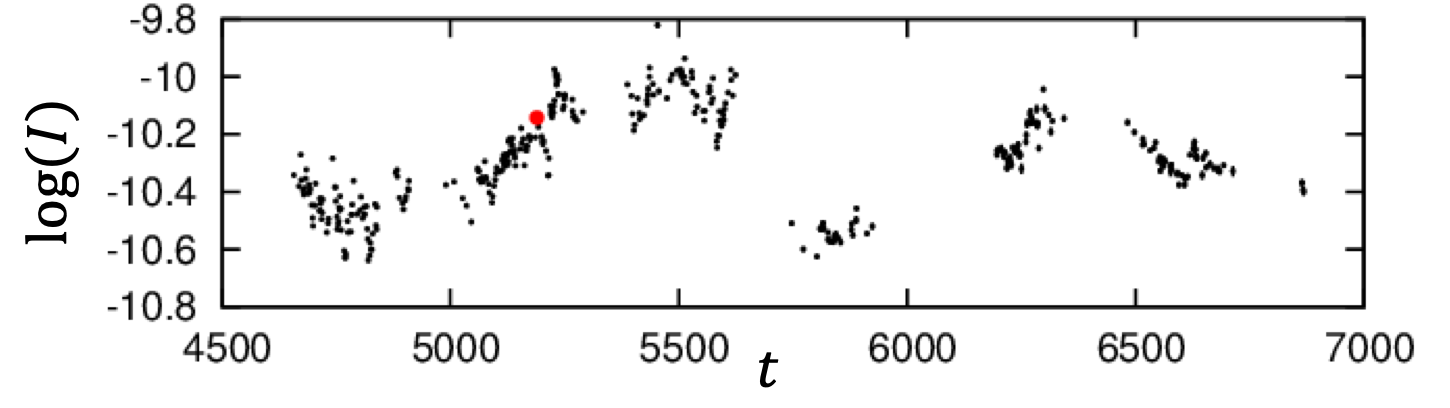
\includegraphics[width=0.75\linewidth]{vgtc_journal_latex/figures/TraditionalMethod_t_I.png}\\
%         \footnotesize{\sf (a)~Light curve ($I$ vs. $t$)}
%     \end{center}
%     \vspace{-5px}
%     \begin{minipage}{0.44\linewidth}
%         \centering
%         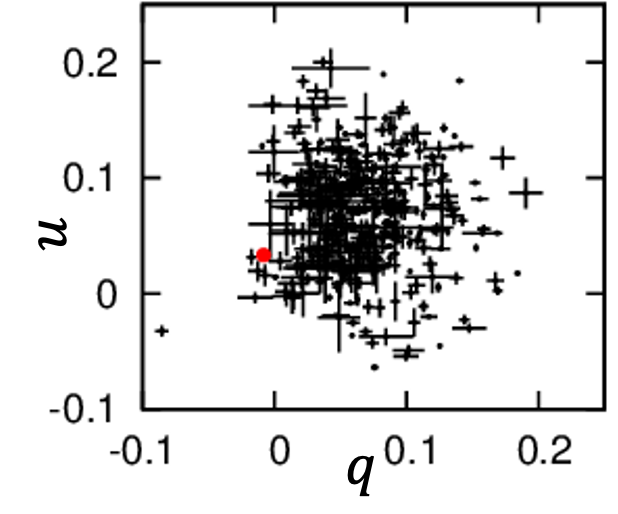
\includegraphics[width=.65\linewidth]{vgtc_journal_latex/figures/TraditionalMethod_q_u.png}\\
%         \footnotesize{\sf (b)~Stokes plane ($u$ vs. $q$)}
%     \end{minipage}
%     \begin{minipage}{0.55\linewidth}
%         \centering
%         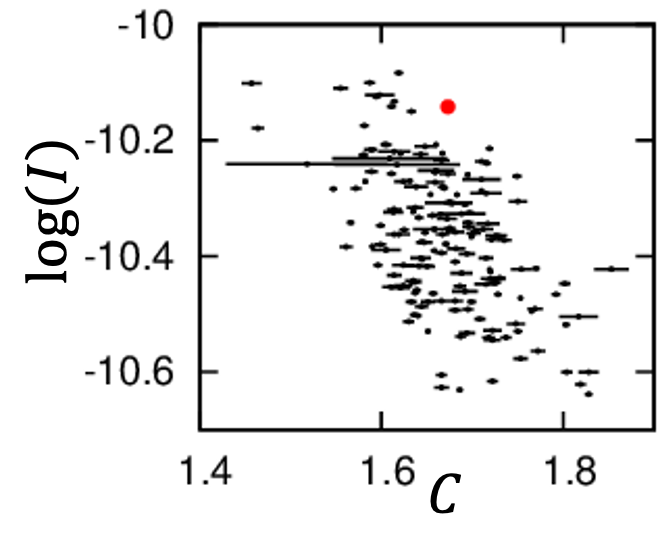
\includegraphics[width=.55\linewidth]{vgtc_journal_latex/figures/TraditionalMethod_c_I.png}\\
%         \footnotesize{\sf (c)~Color–magnitude diagram ($I$ vs. $C$)}
%     \end{minipage}
%     \vspace{-10px}
%     \caption{
%     Animated scatterplots as a conventional way to visualize blazar observations~\cite{Ikejiri2011}. 
%     The plots highlighted in red in sequential order synchronize three scatterplots for cross-reference.
%     }
%     \label{fig:traditionalMethod}
% \end{figure}

\subsection{Visual Exploration Framework\label{sec:approach}}
The design of TimeTubesX supports the visualization tasks outlined in Section~\ref{sec:domainGoalsandTasks}.
Fig.~\ref{fig:framework} illustrates our visual exploration framework.
%
The user workflow starts with visual data fusion~\cite{Fujishiro2018} to create a unified dataset for all subsequent analysis steps (\textbf{T2}).
%All functions can be applied to the unified dataset by visual data fusion~\cite{Fujishiro2018}.
For initial feature and pattern detection (A), users can either rely on automatic feature extraction methods for well-known blazar behaviors (\textbf{T3}) or define their own visual queries for a ROI/SOI (\textbf{T4}, \textbf{T5}).
%For the purpose of the feature extraction, in (A), the user specifies a feature which he/she wants to find out by setting parameters, ROI, or SOI.
The system ranks the results of the feature and pattern detection stage and shows the ranked matches (B).
%the query specified in (A) and shows their overview (B).
Users can sort the results to, for instance, focus on time intervals that have the largest rotation or are the most similar to the input pattern.
%By changing the order of the results, 
%he/she can easily notice which time interval has the biggest rotation 
%or most similar to the input pattern, for instance.
%
% By selecting one or several results of interest, users can analyze, compare, and annotate selected time intervals in more detail (C). 
%By selecting one of the results, he/she may refer to the details of the result and attach an annotation to it if needed (C).
The detailed analysis (C) helps users understand the behavior at the extracted time intervals and classify the results. 
% Annotations allow users to document their analysis process and to share their results with others.
%These details are helpful for him/her understand the the behaviors of the extracted time intervals and
%the annotation supports him/her in recalling his/her analysis process, classify the results, and share the results with other users.
To support iterative refinement of queries, users can build a follow-up query based on the result of a query (D). It allows users to find time intervals similar to the result (\textbf{T4}).
%for another query in the next interactive feature extraction phase (D).
We call this \textit{fact-guided querying}, as it enables users to refine extraction results guided by previously detected features.
To analyze extracted time intervals in more detail, users can employ
the uncertainty-aware TimeTubes view (\textbf{T1}) as well as multiple linked scatterplots views (E).
%He/she can refer to the TimeTubes view as well as the conventional scatterplots view for the extracted time interval with simple interactions (E).
% Our framework supports scatterplots of any two user-defined variables. %, and is linked to the TimeTubes view.
%TimeTubesX can show as many kinds of scatterplots between two arbitrary variables as he/she likes, 
%any of which are federated with TimeTubes view.
%It allows him/her to obtain knowledge or insights on the blazar behaviors.

\textsf{Interactive feature analysis interface.\ } 
% One of the main contributions of TimeTubesX lies in the inherent support for the automatic feature extraction and dynamic visual querying for multi-dimensional, time-dependent blazar datasets.
Fig.~\ref{fig:UIFeatureExtraction} shows our feature and pattern detection user interface. 
The query specification panel (A) allows users %to specify what to extract and 
to build a query with simple interactions either by selecting what to extract, picking a part of data as an input, or sketching time variation patterns.
% In \autoref{fig:UIFeatureExtraction}, (A) shows an on-going query-by-sketch user interaction.
After running a similarity search, 
TimeTubesX ranks and filters extraction results according to the parameters in panel (B),
and then it displays all relevant (i.e., non-filtered) extraction results as a collection of thumbnails in panel (E).
The distance distribution histogram in panel (B) helps users to further filter the number of results.
% which allows users to sort results and to set thresholds for further filtering the number of displayed results.
% To help users set filtering thresholds,
% we use a histogram to provide an overview of the distribution of distances returned by the similarity search.
% By adjusting the gray area on the histogram, users are allowed to alter the number of displayed results. 
The timeline in panel (C) gives an overview of the temporal distribution of the results.
Users are able to recognize groups of results sharing identical time points and temporal distribution features.
% The thumbnails of all relevant (i.e., non-filtered) results are shown in panel (E) to give users an intuitive overview of their query results.
When selecting an individual thumbnail, TimeTubesX shows a detailed information on the corresponding result in panel (D), including exact time stamps and the distance between the query and the result.
% The detailed information is helpful for users' deeper understanding of the extracted time interval.
To re-utilize the query, compare multiple query results, and share the query and their results with other users, 
TimeTubesX allows users to export and import queries and their results in the form of JSON files (a custom format for TimeTubesX).
When importing previous query results,
panel (F) shows a summary of the query used in the previous process and panel (C) shows another timeline for the imported query results.

Fig.~\ref{fig:querySpecificationPanel} shows the query specification panels for each mode of the feature and pattern detection.

% MERGED VERSION
% The design of TimeTubesX supports the visualization tasks outlined in \autoref{sec:domainGoalsandTasks}.
% \autoref{fig:framework} illustrates our visual exploration framework, while \autoref{fig:UIFeatureExtraction} shows our feature and pattern detection user interface.
% The visual exploration workflow starts with visual data fusion~\cite{Fujishiro2018} to create a unified dataset for all subsequent analysis steps (\textbf{T2}).
% For initial feature and pattern detection in \autoref{fig:framework}~(A), users can either rely on automatic feature extraction methods for well-known blazar behaviors (\textbf{T3}) or can define their own visual queries for a ROI/SOI (\textbf{T4}, \textbf{T5}).
% The query specification panel in \autoref{fig:UIFeatureExtraction}~(A) allows users to specify what to extract and to build a query with simple interactions.
% As the next step, the system ranks the results of the feature and pattern detection stage and shows the ranked matches, as illustrated in  \autoref{fig:framework}~(B).
% Users can sort the results, e.g., to focus on time intervals that have the largest rotation or are the most similar to the input pattern.
% They are allowed to choose in what order to sort the results and set thresholds for further filtering the number of displayed results with the suggestion of a distance distribution histogram in \autoref{fig:UIFeatureExtraction}~(B).
% % By adjusting the gray area on the histogram, users are allowed to alter the number of displayed results.
% They can overview the temporal distribution of all relevant (i.e., non-filtered) extraction results through the timelines in \autoref{fig:UIFeatureExtraction}~(C) and the thumbnails of sorted results in \autoref{fig:UIFeatureExtraction}~(E).
% The detailed analysis in \autoref{fig:framework}~(C) helps users deeply understand the behavior of the extracted time intervals and classify their results. 
% \autoref{fig:UIFeatureExtraction}~(D) shows detailed information on a selected result, including exact time stamps and the distance between the query and the result.
% To support iterative refinement of queries, users can build a follow-up query based on the result of a query, as illustrated in \autoref{fig:framework}~(D). 
% It allows users to identify time intervals similar to the result (\textbf{T4}).
% We call this \textit{fact-guided querying}, as it enables users to refine extraction results guided by previously detected features.
% To analyze extracted time intervals in more detail, users can employ
% the uncertainty-aware TimeTubes view (\textbf{T1}) as well as multiple linked scatterplots views, as shown in \autoref{fig:framework}~(E).
% Our framework supports scatterplots of any two user-defined variables. 
% To compare multiple query results,
% TimeTubesX allows users to export and import query results.
% When importing previous query results,
% \autoref{fig:UIFeatureExtraction}~(F) shows a summary of the query used in the previous extraction process, and \autoref{fig:UIFeatureExtraction}~(C) shows another timeline for the imported query results.

To better demonstrate our feature and pattern detection methods, we will use a synthetic dataset (see Fig.~\ref{fig:synthesisData}) as a running example in Sections~\ref{sec:automaticExtraction} and \ref{sec:visualQuery}.
%for illuminating the feature extraction, as illustrated in \autoref{fig:synthesisData}.
It contains four large peaks in $I$, as highlighted by orange diamonds in (a), three small red circular patterns on the Stokes plane in (b), three large green rotations , and three narrow/rough-edged blue patterns.

% \begin{figure}[H]
%     \centering
%     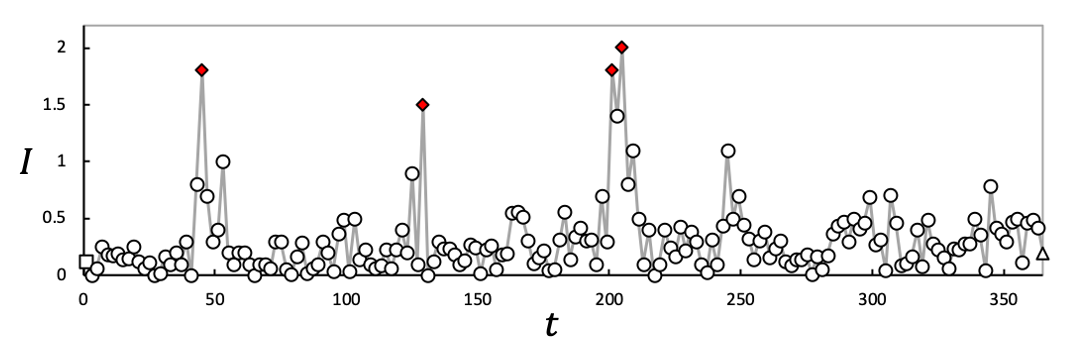
\includegraphics[width=.8\linewidth]{vgtc_journal_latex/figures/synthesisDataLightCurveLabel.png}\\
%     \footnotesize{\sf (a) Light curve plot. The four red diamonds indicate peaks in the data.}\\
%     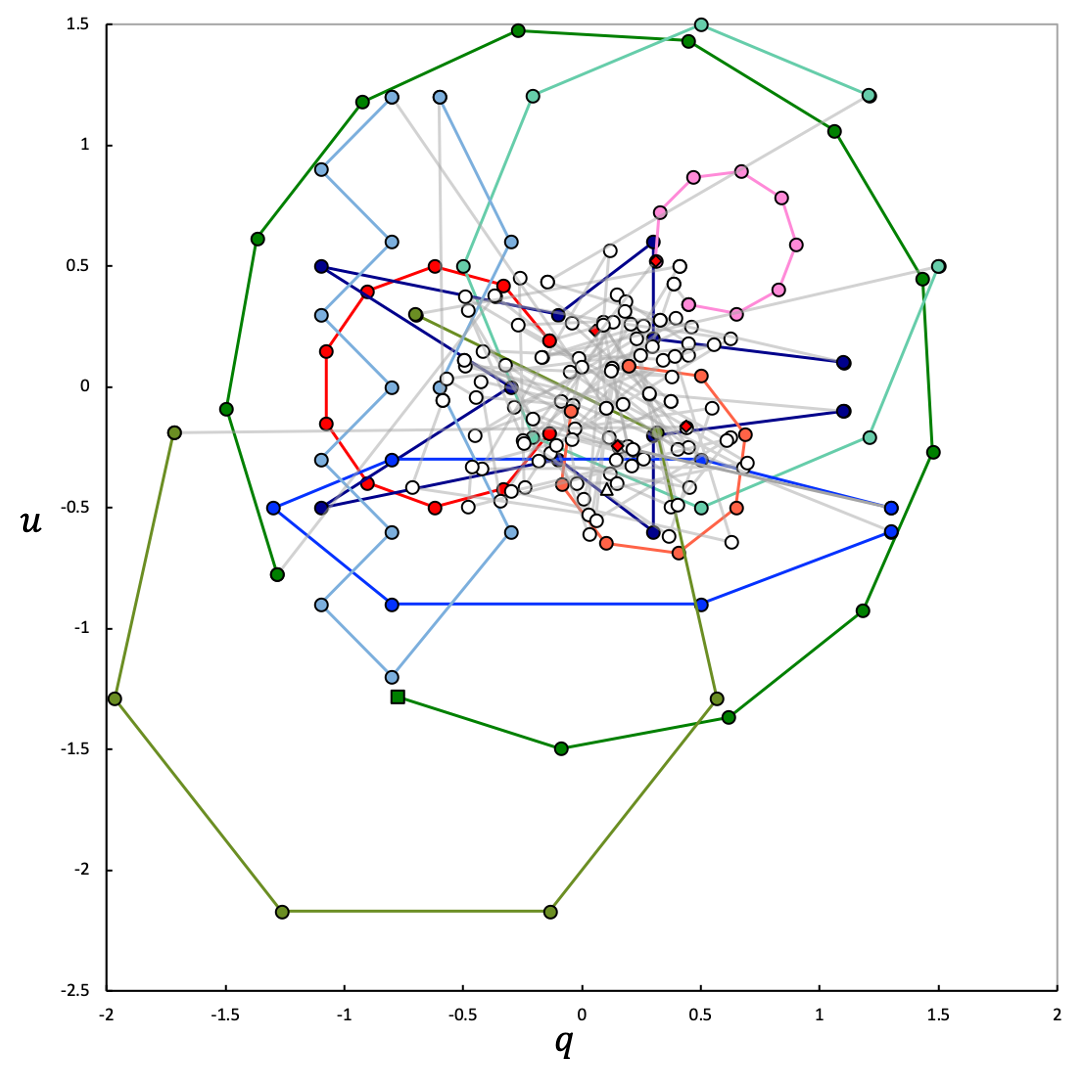
\includegraphics[width=.83\linewidth]{vgtc_journal_latex/figures/synthesisDataStokesLabel.png}\\
%     \footnotesize{\sf (b) Stokes plane plot. The red diamonds indicate the peaks shown in (a).}
%     \caption{Conventional stokes plane and light curve plots for our synthetic dataset. The data includes three small circular patterns (red), three big rotations (green), and three narrow/rough-edged patterns (blue) within 365 days. Data starts from a square plot and ends at a triangular plot.}
%     \label{fig:synthesisData}
% \end{figure}


% \begin{figure*}[t]
%     \centering
%     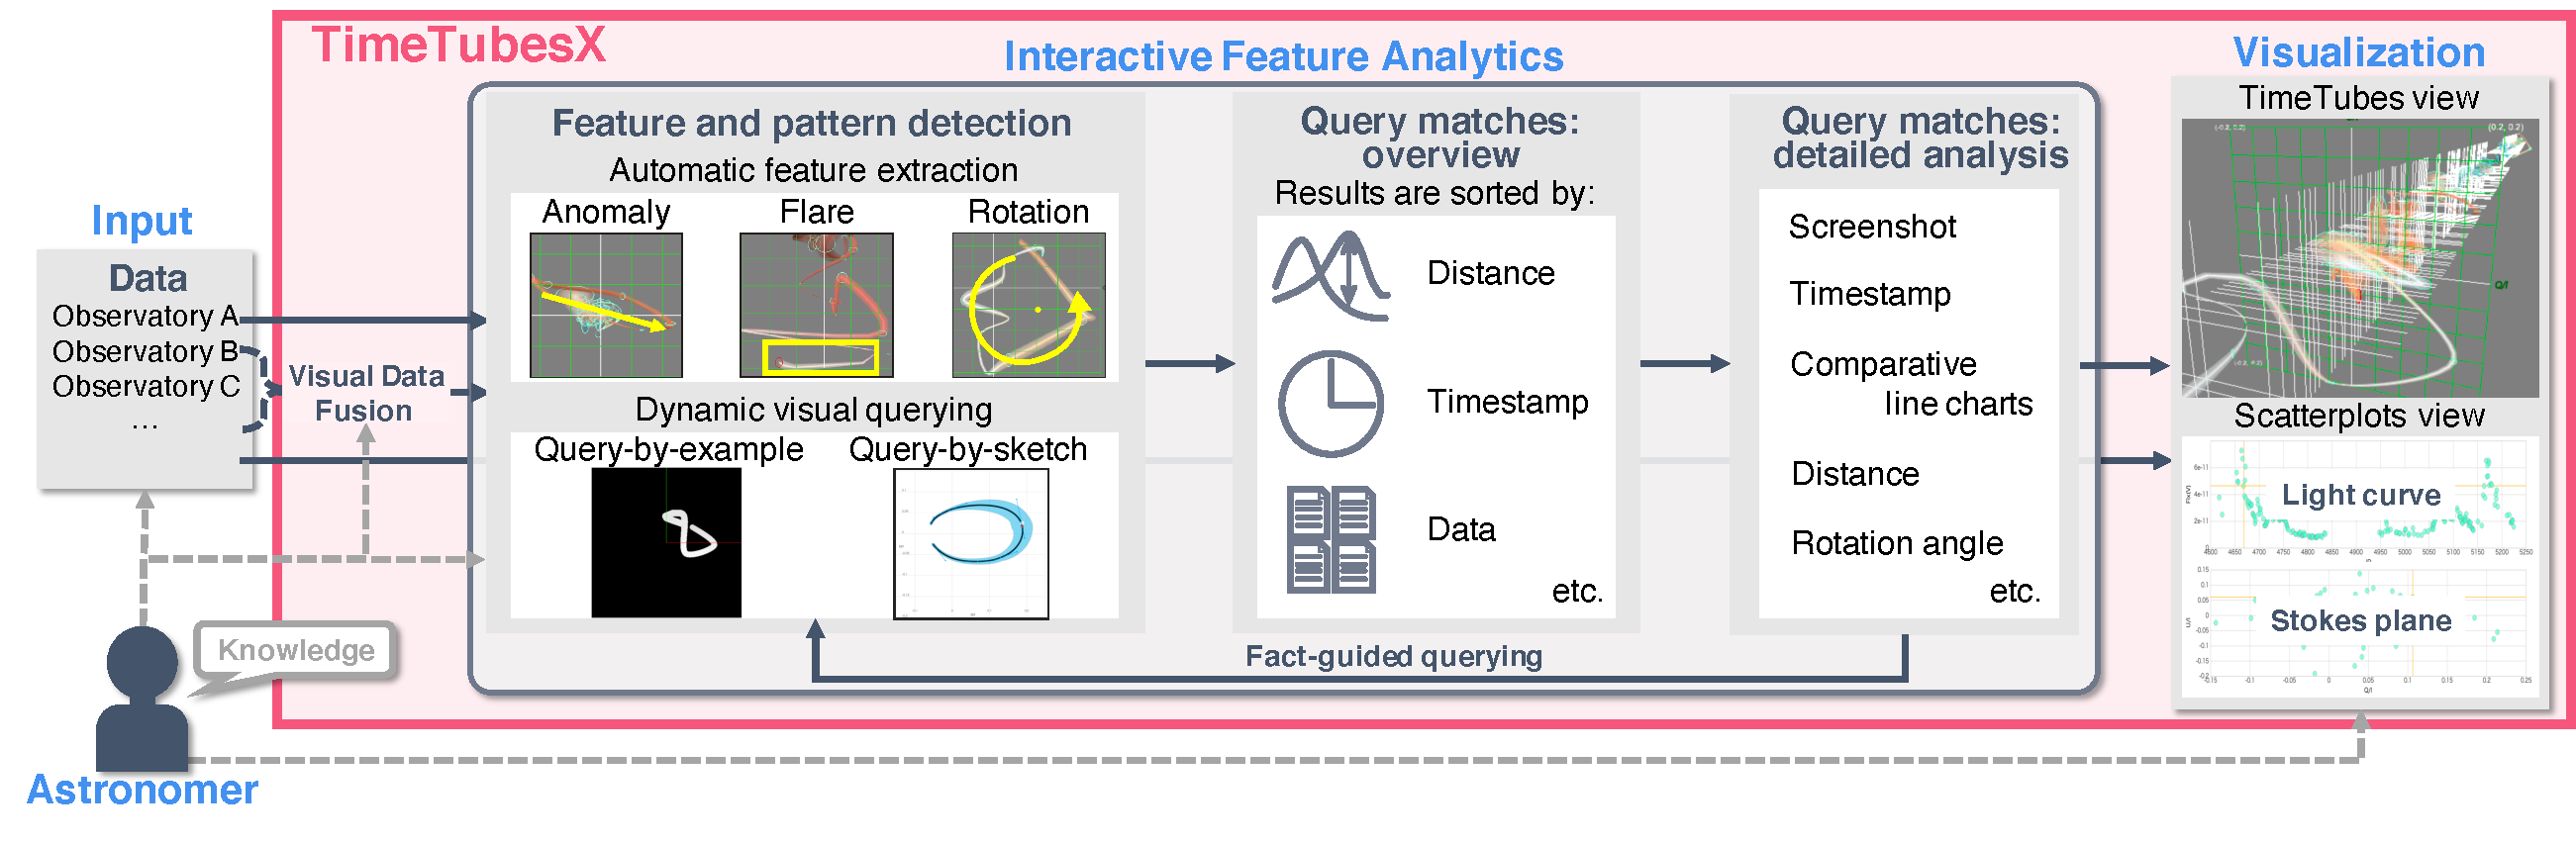
\includegraphics[width=0.9\textwidth]{vgtc_journal_latex/figures/workflowGray.pdf}
%     \caption{Visual exploration framework of TimeTubesX. TimeTubesX can deal with multiple input datasets through visual data fusion. (A)~The user specifies what to extract; (B)~Extraction results are ordered by an arbitrary property; (C)~Detailed information of a selected result is provided; (D)~An extracted result can be re-utilized for another query in the interactive feature extraction; (E)~The user is allowed to refer to TimeTubes view or scatterplots view for the extracted time interval and explore it with various exploration functions.}
%     \label{fig:framework}
% \end{figure*}
% We newly introduce two types of feature extraction into TimeTubesX: automatic and interactive.
% The automatic feature extraction can extract notable time intervals to meet given specifications,
% whereas the interactive feature extraction can find out time intervals similar to a given ROI or SOI. 

% TODO: Move the following part to the introduction?
% Regarding the behaviors of blazars, there are a lot of mysterious parts. 
% When the relativistic jet in a blazar forms a burst, the light from a blazar gets highly luminous, that is called a flare. 
% Flare is one of the most characteristic behaviors. 
% Some astronomers report that the polarization direction of the light from blazars sometimes rotates. 
% However, it is controversial in astronomy whether the rotations are real ones or fake ones caused by random variations of polarization.
% To verify polarization rotations, astronomers need to scrutinize correlations among other observation variables. 
% On the other hand, there can exist undiscovered phenomena of blazars. 
% It is significant to explore recurring patterns of time variations or correlations among variables. 
% Nevertheless, deliberate analysis across multiple variables is indispensable.
% To address these difficulties, we introduce a novel feature extraction for blazar observations.
% It supports two types of feature extraction: Automatic extraction and visual query. 
% The automatic extraction can squeeze only observable time intervals from (multiple) long-term observations, 
% whereas the visual query can find time intervals similar to a region of interest (ROI) or shape of interest (POI). 
% The feature extraction can deal with visually fused datasets.

% It allows him/her to deeply understand blazar behaviors and obtain knowledge or insights on them.
% Note that task \textbf{T2} is supported by all the functions of the feature extraction.

% The following sections (Sections~\ref{sec:automaticExtraction}, \ref{sec:visualQuery}, and \ref{sec:otherFunctions}) detail functions involving the feature extraction.